% !TEX root = DesignDocument.tex


\chapter{Research Results}

%%This chapter describes the results and conclusions of your research.   This would be the final report for a research project.  

By the conclusion of the project, many different results had been drawn about several aspects of the cluster. The first are the results of testing of each single device. Then, the maximum amount of Gigaflops the cluster can produce with LINPACK was found. GPIO and USB communication were also analyzed. 

\section{Result 1}

First, the Raspberry PI 2B and ODROID XU4 were tested individually to find which was faster. The results are shown in Figure~\ref{pivodroid} along with the final metric of Gigaflops per dollar per watt. It was found that the Raspberry Pi cost \$35 and used 4 watts of power while running, and the ODroid cost \$75 and used 15 watts. 

\begin{figure}[tbh]
\begin{center}
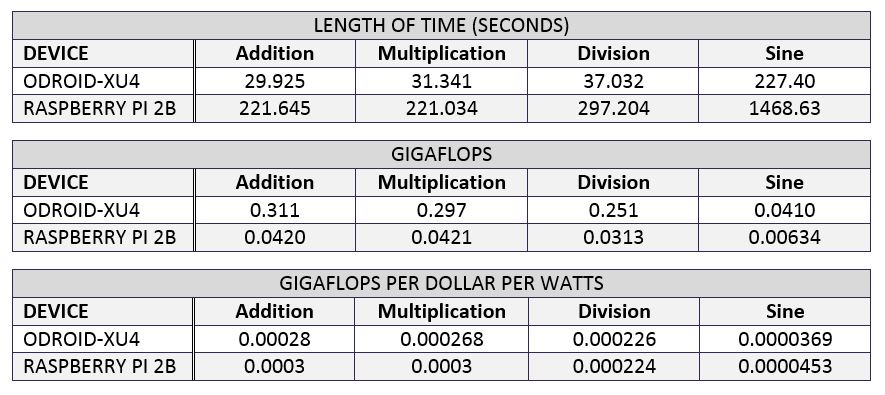
\includegraphics[width=0.75\textwidth]{pivsxu4table2.JPG}
\end{center}
\caption{PI vs ODROID results. \label{pivodroid}}
\end{figure}

\section{Result 2}

We also measured the speed of the Ethernet connections using the tool iperf. It was testing by directly connecting two devices Ethernet to Ethernet, and connected over the switch. Also, using USB to Etherent devices to create new network interfaces on the ODroids was tested by connecting those ports to the built in Ethernet ports. The results are shown in Table~\ref{ethernet}

\begin{table}[tbh]
\caption{Ethernet speeds. \label{ethernet}}
\begin{center}
\begin{tabular}{|r|l|}
  \hline
  Ethernet to Ethernet & 750 Mbps \\
  USB to Ethernet &  450 Mbps \\ 
  Ethernet over switch & 750 Mbps \\
  \hline
\end{tabular}
\end{center}
\end{table}

\section{Result 3}

Direct USB to USB communication was also tested. The devices were attached by USB 3.0 ports with the intent to use them to pass information between. However, further research proved that there is no current way to transfer information from two hosts using USB 3.0. It can be done with USB 2.0 using crossover cables, but there does not exist any common operating system that supports the same feature with 3.0. Therefore, we did not benchmark USB 3.0 communication.

\section{Result 4}

Another alternate form of communication tested was GPIO. The library WiringPi was installed and used with C to read and write values to pins. It was found that communication was successful, but in order to make a protocol faster than Ethernet, even if we used all 40 pins to tranfer data, we would need each pin to send over 19.5 million bits per second, as per \begin{equation}(750 * 1024^{2}) / 40 \end{equation}WiringPi, in our preliminary testing, was only able to send about 500,000 bits per second on a pin. Therefore, it was concluded that our cluster would always be faster using Ethernet.

\section{Result 5}

Our final result was using LINPACK to test the amount of Gigaflops produced by the cluster. First we configured and ran the test on a single device using all four of the A7 cores. We found that the maximum was 3.05 Gigaflops. Then, with the cluster in a star topology, we increased the amount of nodes we ran LINACK on up to all eight, and the results are graphed in Figure~\ref{linpackresults} The most Gigaflops we were able to get from the A7 cores on all of the ODROIDS together was 13.38.

\begin{figure}[tbh]
\begin{center}
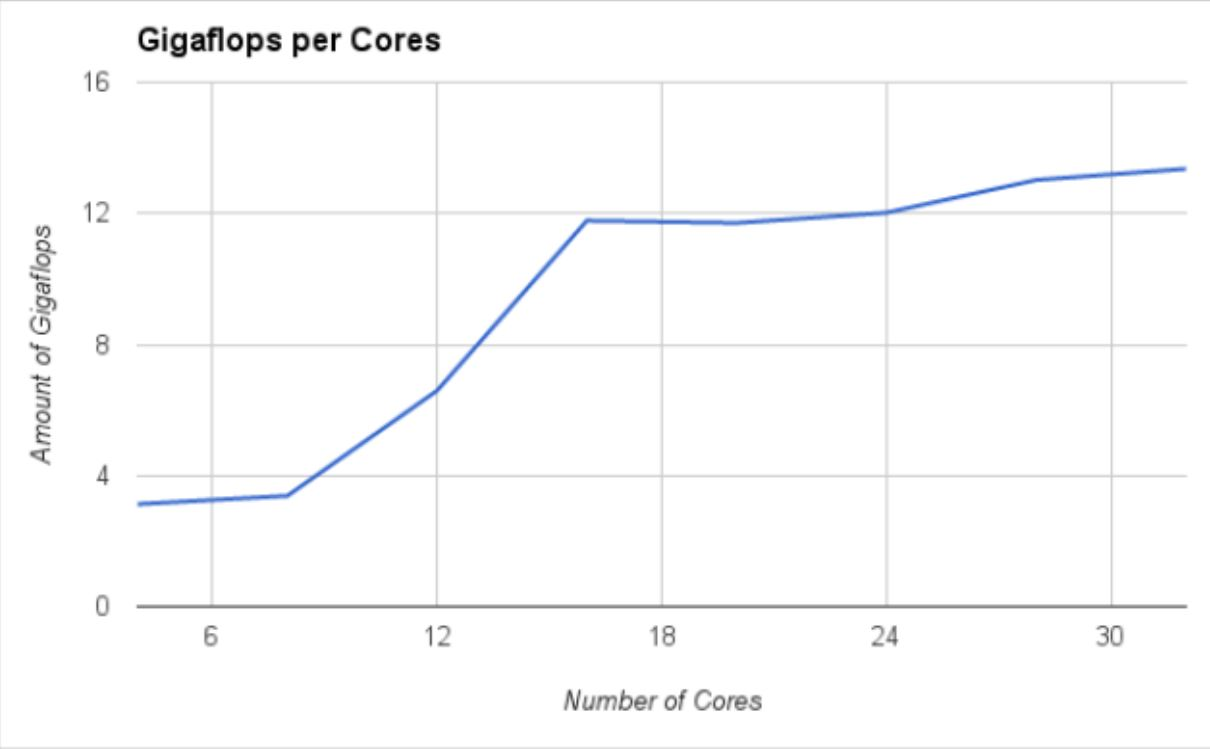
\includegraphics[width=0.75\textwidth]{minimalgraph.JPG}
\end{center}
\caption{LINPACK results. \label{linpackresults}}
\end{figure}

The next step was to use the A15 cores. This proved to be difficult as described earlier, due to the operating system preferring to use the A7 cores and providing no user control over proccess affinity. However, we were able to get a few results out of the A15s as shown in Table~\ref{a15} The HTOP utility was used to confirm that the A15 core were indeed being used. 

\begin{table}[tbh]
\caption{A15 core speed. \label{a15}}
\begin{center}
\begin{tabular}{|r|l|}
  \hline
  1 core per node &  17.05 Gigaflops \\
  2 core per node &  26.23 Gigaflops \\ 
  \hline
\end{tabular}
\end{center}
\end{table}

\section{Result 6}

We also benchmarked a standard i7 desktop using LINPACK, specifically Dr. Karlsson's, for a point of comparison to our cluster. It had four hyperthreaded cores for a total of eight different processes that can be running simultaneously. The total cost of this machine was roughly comprable to the total cost of our cluster, so it made sense to compare the computational power of the two. We found the i7 desktop machine to be able to produce about 61 Gigaflops. 

\section{Conclusions}

In conclusion, we found that Ethernet was the fastest communication method we had availible. We were able to transfer data at a rate of roughly 750 Mbps. In comparison, GPIO communication with WiringPi was only able to send 0.5 Mbps per pin. Even with all 40 GPIO pins, communication protocols we would write ourselves with GPIO would be significantly slower than Etherent. USB to USB communication did not work at all.

When using a star topology, with all ODROIDS running four processes each and using their A7 cores, for a total of 32 cores, the speed was 13.38 Gigaflops, whereas only two A15 cores on each device for a total of 16 cores produced 26.23 Gigaflops. Clearly, the A15 cores are drastically more powerful than the A7s. If we were able to force the ODROIDS to use all four of their availible A15s, it is likely that the performance of our cluster would be roughly 48 Gigaflops from the four A15s, if the pattern of increase stayed consistent. That combined with the 13.38 from the A7s would produce an approximate total of about 60 Gigaflops. This would be comprable to the performance measured from Dr. Karlsson's i7 machine.

\section{Further work} 

In order to gather more results in the future, we would ideally be able to benchmark the cluster with a ring and hypercube topology. This would require one of two things, the first option being to find a way to run LINPACK and MPI code over devices with multiple network interfaces. Once that was done, it would be possible to run the tests in the exact same configuration as was done for the star topology through the switch. An alternative solution would be to find a different benchmarking method entirely. The disadvantage would be the increased workload of running that new benchmark on all of the previous tested configurations we have done up to this point.

Another goal for the future would be to benchmark all of the A15 cores. Since we were able to use one and two of them per node, it's clearly possible for them to be used, the difficutly lies with getting the operating system to schedule the LINPACK processes to those cores. This would involve more testing to see exactly when the OS did use the A15s and find a way to repeat it.

As well as gathering more data on the performance of the cluster, more uses for the project include testing real life problems. This could include things such as the traveling salesman problem, a well known problem that can only be solved with brute force and takes a large amount of computation to solve. The cluster would be used to determine how quickly it can solve the problems, and how to most effeciently divide up the problem to solve it with parallelization.
